\section{Metodología}
\label{sec:metodologia}
\subsection{Morfología de las shells de la BCG de \clust{}} \label{sec:contorno}
\nota{no tengo muy claro si usar el presente o el pasado para describir los pasos}
El primer objetivo que nos debemos marcar es la delimitación de las regiones del espacio cercano a la BCG en las que existen shells. Como explicamos en la introducción, las shells se pueden considerar como excesos de luminosidad que alteran la curva de luz de una galaxia. Por lo tanto, una forma sencilla de aislar la luz producida por las shells es proponer un modelo \enquote{de primer orden} para el perfil luminoso de la BCG y considerar únicamente la luz sobrante, en lo que llamamos la imagen residual. El software GALFIT \citep{pengDetailedStructuralDecomposition2002, pengDETAILEDDECOMPOSITIONGALAXY2010} es capaz de ajustar los parámetros de dicho modelo y devolver una imagen, a priori, sin la luz de la BCG. El perfil de luz más común para una galaxia elíptica es el llamado perfil de Sérsic \citep{sersicInfluenceAtmosphericInstrumental1963,savorgnanSupermassiveBlackHole2013}, que tiene la siguiente forma \citep{pengDetailedStructuralDecomposition2002}:

\begin{equation}
    \Sigma (r) = \Sigma_e e^{-\kappa [(r/r_e)^{1/n} - 1]}
\end{equation}

donde \(\Sigma (r)\) representa el brillo superficial en el radio elíptico \(r\); \(r_e\) el radio que encierra la mitad de la luz emitida por la galaxia; \(\Sigma_e\) el brillo superficial en \(r_e\); \(n\) el índice de Sérsic, que determina la concentración de la luz (un índice más alto implica una transición más abrupta entre el núcleo brillante de la galaxia y el halo tenue, característico de las galaxias elípticas); y \(\kappa\) un parámetro dependiente de \(n\) que mantiene constante la relación de \(r_e\) con el flujo. \par

Siguiendo esta idea, vamos a ajustar la BCG de \clust{} con un perfil de Sérsic elíptico y unos parámetros iniciales para su tamaño, forma y brillo obtenidos con la ayuda de SAOImage DS9. Para ello seleccionamos, por su resolución, las imágenes de JWST, y de entre ellas la del filtro F277W, por ser la más brillante que no presenta wisps. El modelo producido por el ajuste de GALFIT es una elipse con las siguientes características: centro situado a \(21^{\text{h}}29^{\text{m}}39^{\text{s}}.9573\) de ascensión recta y \(+00^{\circ} 05^{\prime}21^{\prime\prime}.24\) de declinación; \(r_e = 12,41 \: \text{arcsec} \: (46,20 \: \text{kpc})\); \(n = 3,03\); \(b/a = 0,51\) y \(\alpha = 64,75^{\circ}\); donde \(b/a\) es el cociente entre ejes de la elipse y \(\alpha\) el ángulo del eje mayor con respecto a la vertical. El ajuste tiene un \(\chi^{2}_{\nu} = 0,602\) y se mantiene estable ante grandes variaciones de los parámetros iniciales, lo que sugiere que es robusto. En la fila superior de la figura \ref{jwst277} incluimos, con la misma escala que en la figura \ref{bcg} (0-1 MJy/sr), la imagen de JWST de la BCG y el modelo de GALFIT. En la primera imagen observamos, además de las estructuras que ya comentamos para la figura \ref{bcg}, varios posibles casos de galaxias afectadas por \textit{lensing} (lentes gravitatorias). Al este de la BCG tenemos el ejemplo más claro, con una galaxia claramente duplicada y cuya luz forma un arco de anillo de curvatura amplia. Más sutiles son las dos galaxias que se encuentran al sur de la BCG, que, pese a que la imagen no es concluyente, parecen sufrir el mismo fenómeno. Por su parte, en el modelo de GALFIT tenemos una elipse cuya forma y brillo coinciden a grandes rasgos con los de la BCG, señal de que el ajuste es acertado. \par 

La tercera imagen de la figura se corresponde con el resultado de restar la elipse del modelo a la imagen original. Para resaltar las regiones de bajo brillo superficial, se representa con una escala de 0 a 0,2 MJy/sr. De inmediato se distingue una shell al este de la BCG, en la región donde están presentes las galaxias que ya veíamos antes. También se aprecia, en el lado opuesto, una zona luminosa mucho más delgada y tenue que cumple las características de una shell. Por lo tanto, este modelo simple permite identificar dos shells en la imagen del filtro F277W de JWST. Es probable que la luz restante al noroeste de la BCG también se corresponda con varias shells. De hecho, se intuye la presencia de picos y valles de luminosidad, característicos de estas estructuras. Sin embargo, en la imagen residual no es posible distinguir todo el arco de las shells, si es que este existe, por lo que no las vamos a considerar. Por último, en esta imagen también se destaca una de las galaxias (la más occidental) al sur de la BCG afectadas por \textit{lensing} que señalábamos en el párrafo anterior. La más oriental no tiene un anillo identificable en esta imagen, pero sí se distinguen los puntos más brillantes en los extremos (correspondientes con una imagen duplicada de la galaxia), lo que refuerza esta observación. \par


\begin{figure}[h]
\centering
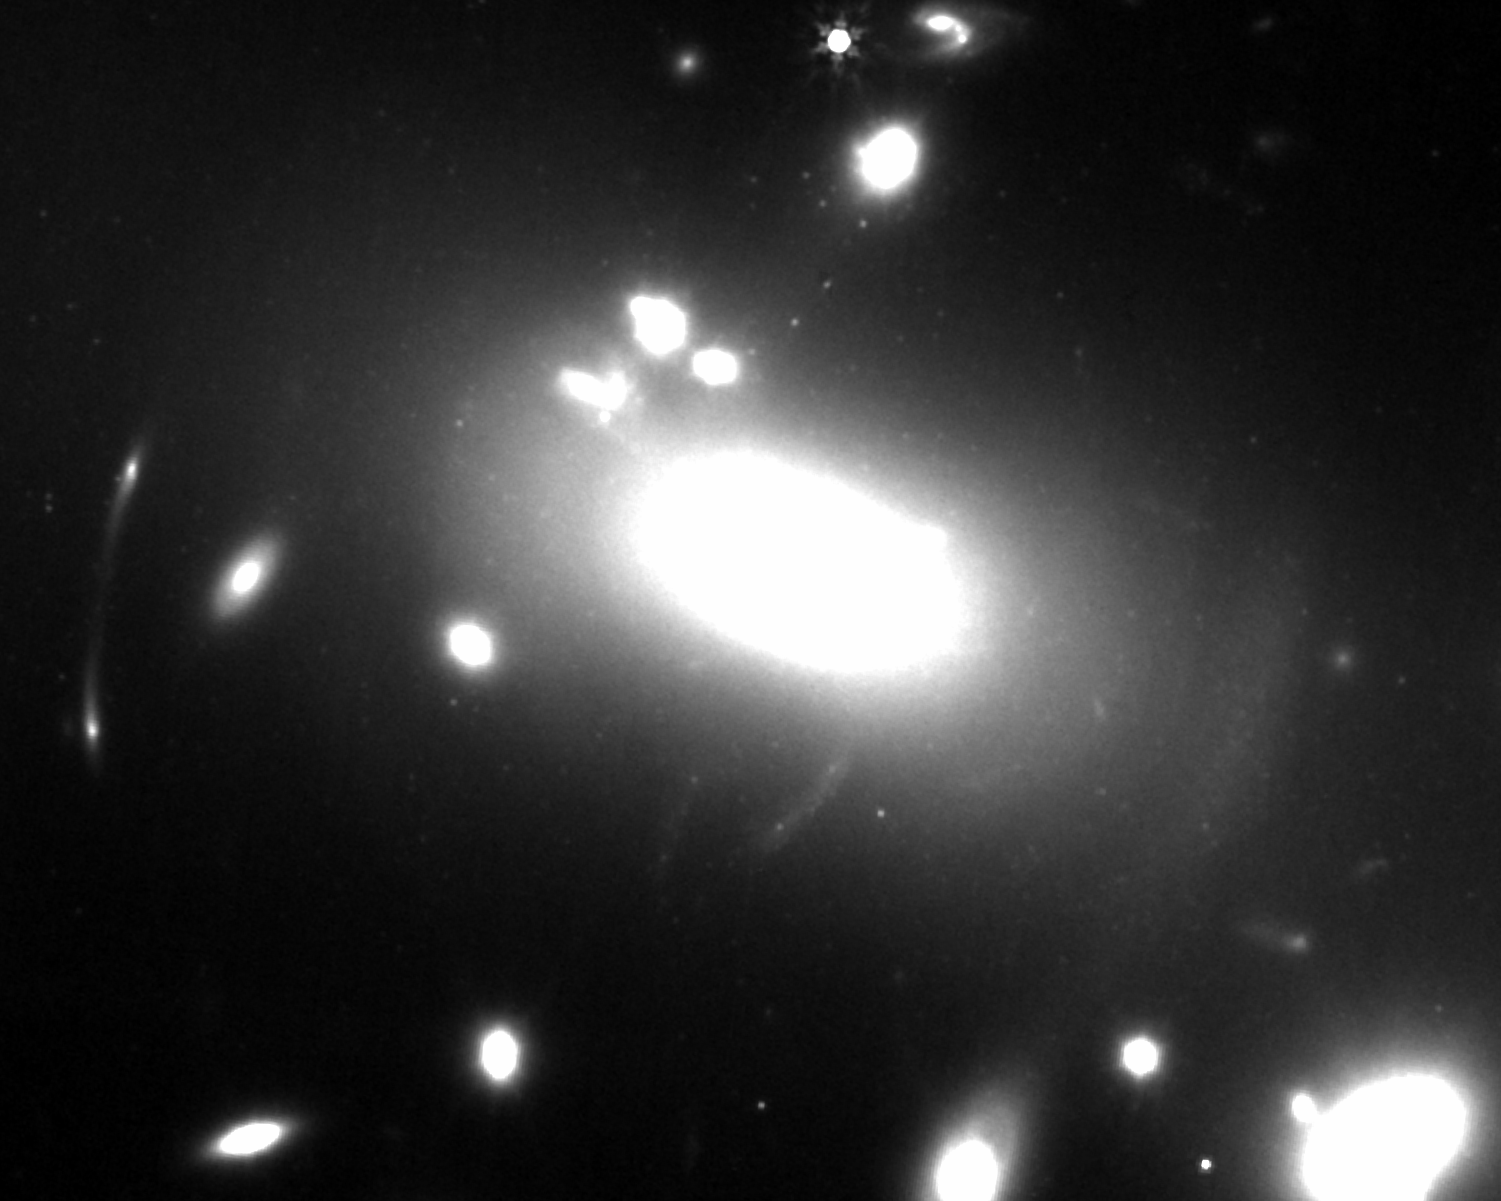
\includegraphics[trim={0 0 0 0}, clip, width=0.45\textwidth]{jwst277.png}
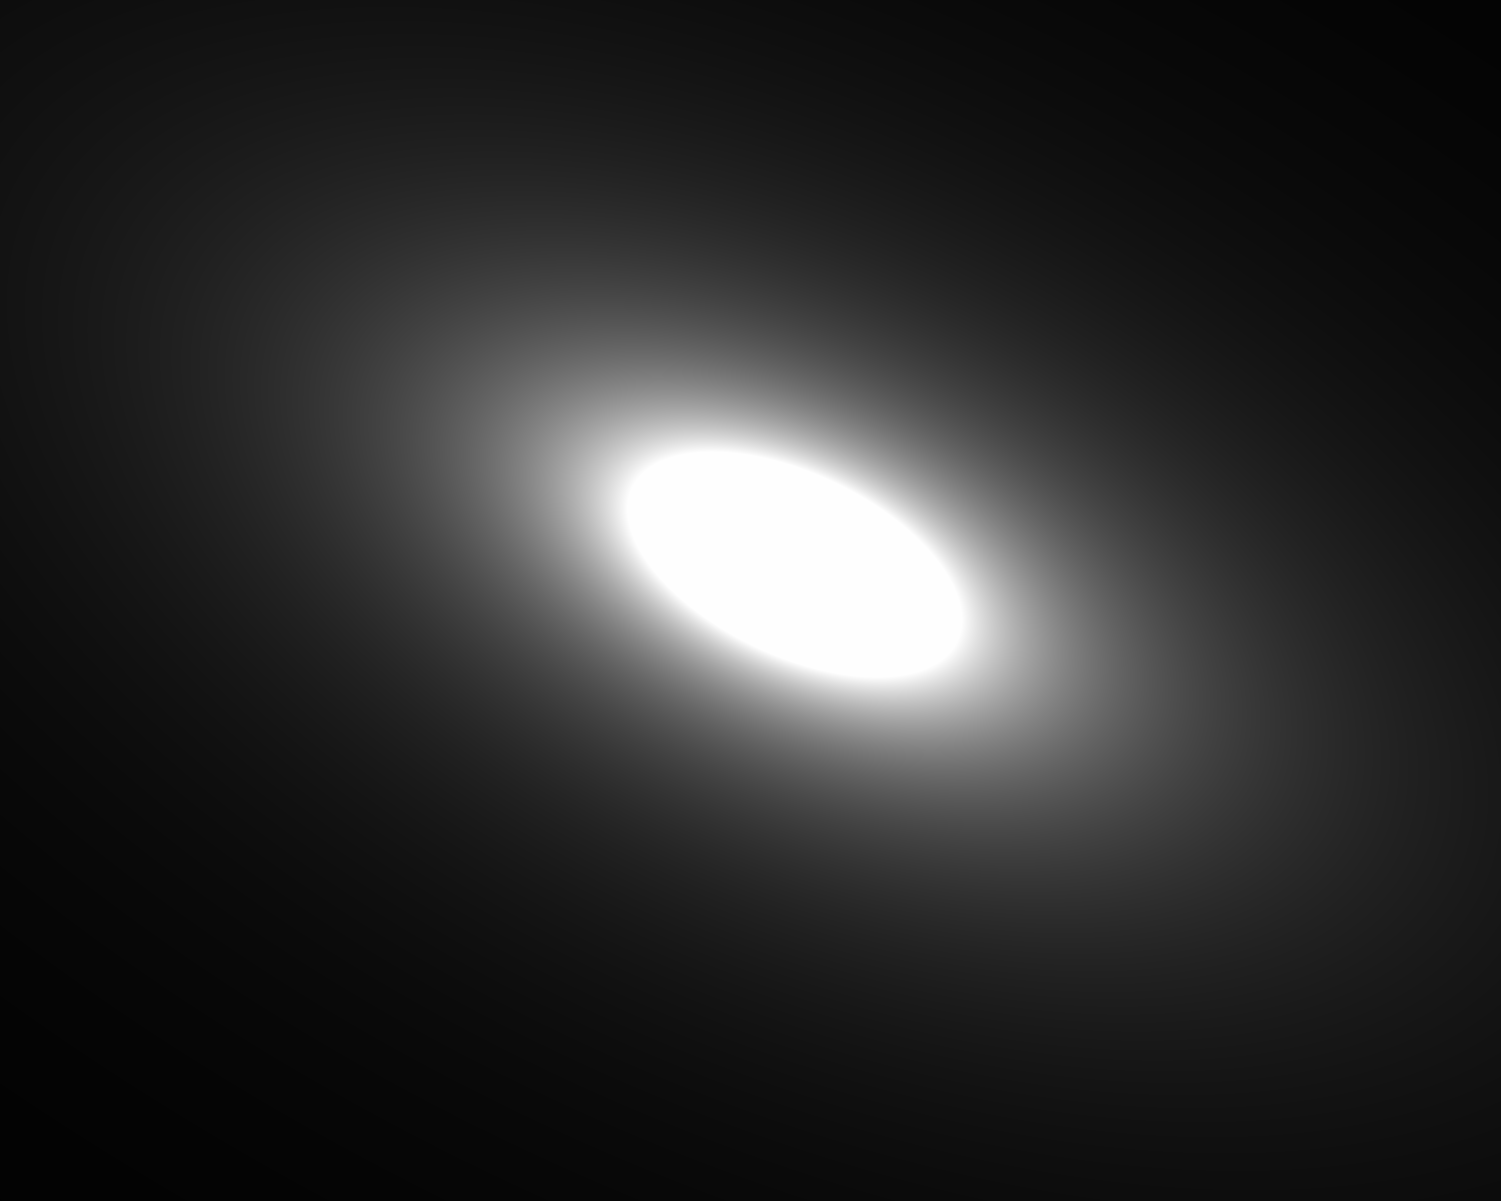
\includegraphics[trim={0 0 0 0}, clip, width=0.45\textwidth]{jwst277_elipse.png} \\
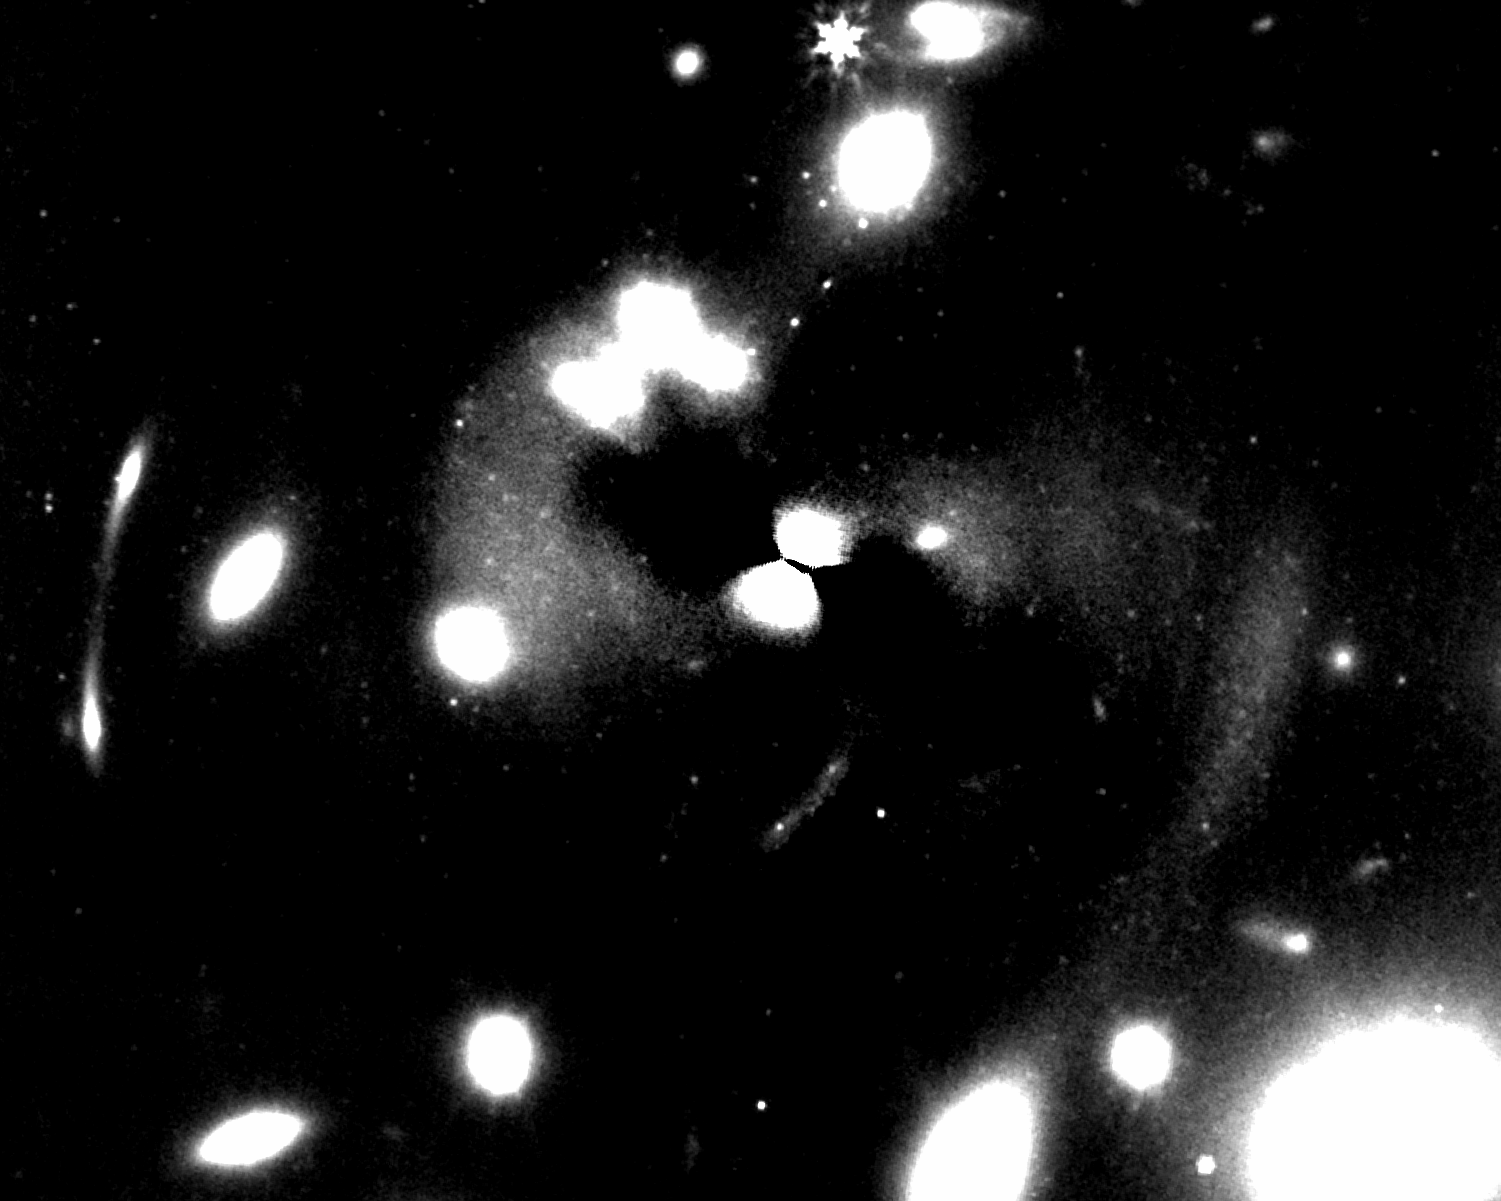
\includegraphics[trim={0 0 0 0}, clip, width=0.5\textwidth]{jwst277_sinbcg.png}
\caption{Fila superior, izquierda: imagen ampliada de la BCG de \clust{} en el filtro F277W de JWST con una escala de 0-1 MJy/sr, descrita en el texto. Fila superior, derecha: modelo de GALFIT de la BCG de \clust{}, con la misma escala. Se observa un contorno y un brillo muy similar. Inferior: imagen residual resultante de restar la segunda imagen a la primera, con una escala de 0-0,2 MJy/sr. Como se indica en el texto, se aprecian claramente dos shells, y hay indicios de que existen más.  \label{jwst277}}
\end{figure}
\noindent

Aplicando el mismo procedimiento para las demás imágenes de JWST, comprobamos que se obtienen resultados muy similares para todas ellas. Por lo tanto, llegados a este punto parece razonable plantear un análisis en el que se elimine la luz de la BCG en cada filtro y se midan las características de las shells aisladas. Sin embargo, en las imágenes de HST el ajuste es problemático. En la figura \ref{hst160} aplicamos el mismo procedimiento que en la figura \ref{jwst277} a la imagen del filtro F160W. En este caso, GALFIT modela una galaxia más alargada (\(b/a = 0,38\) ) que hace desaparecer la shell occidental y afecta gravemente al centro de la oriental. Además, no es capaz de eliminar satisfactoriamente la luz de la BCG al norte y al sur, por lo que tampoco es posible distinguir esta shell de la BCG. Este ajuste es estable bajo grandes variaciones de los parámetros iniciales y la aplicación de máscaras (zonas no tenidas en cuenta en el ajuste) en determinadas regiones. \par

\begin{figure}[h]
\centering
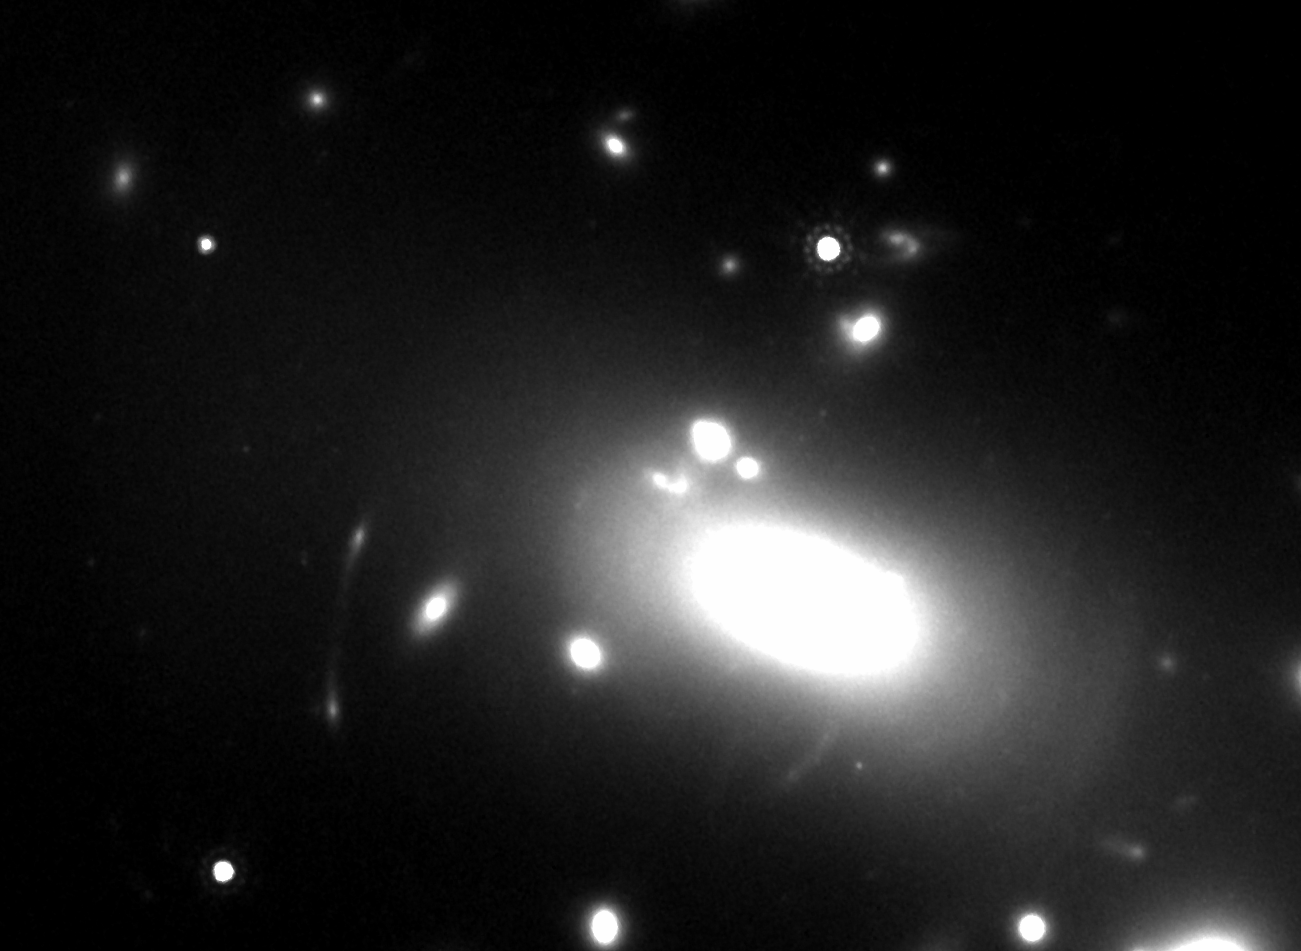
\includegraphics[trim={300 0 0 200}, clip, width=0.45\textwidth]{hst160.png}
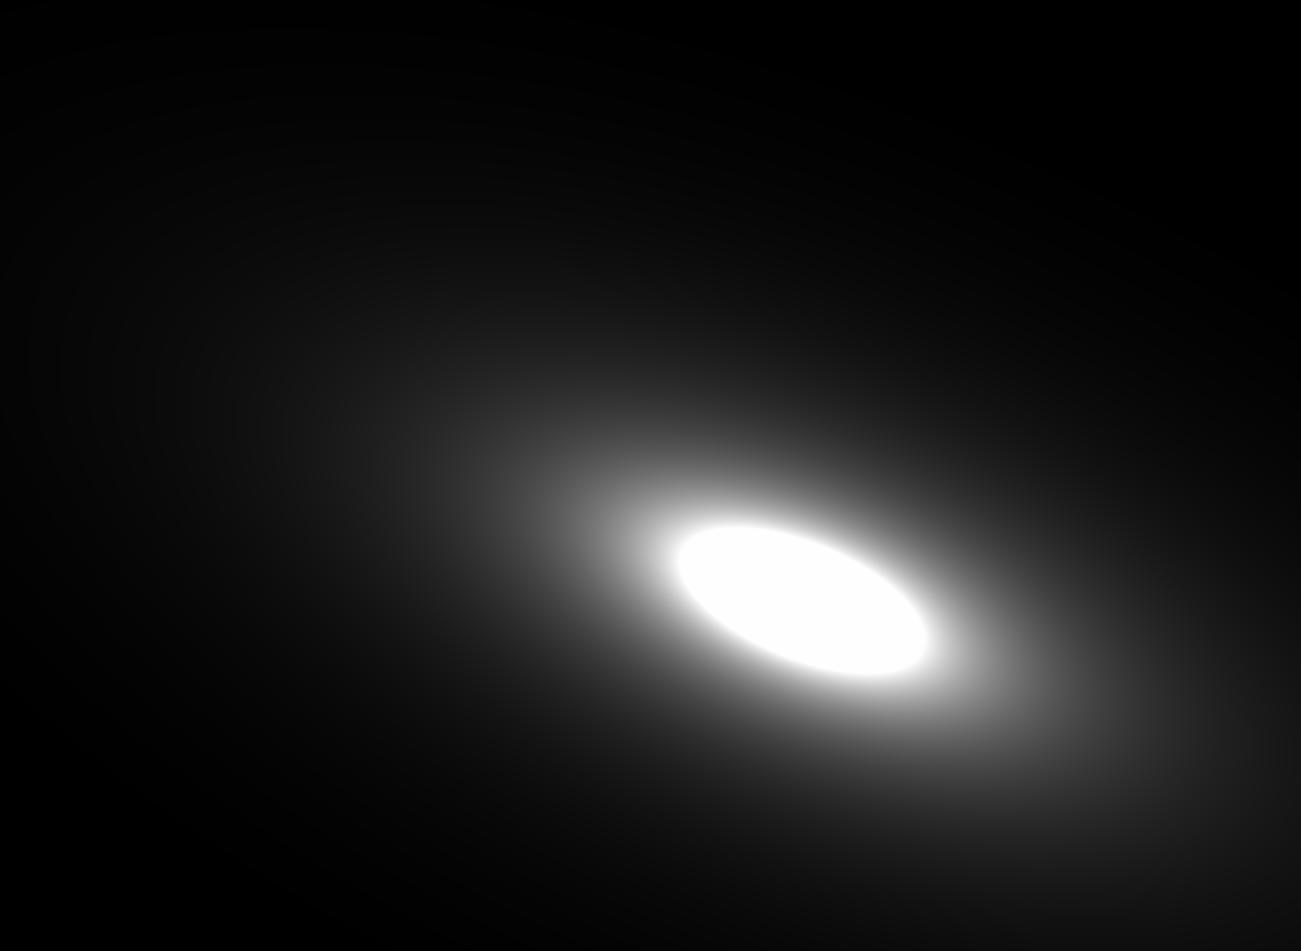
\includegraphics[trim={300 0 0 200}, clip, width=0.45\textwidth]{hst160_elipse.png} \\
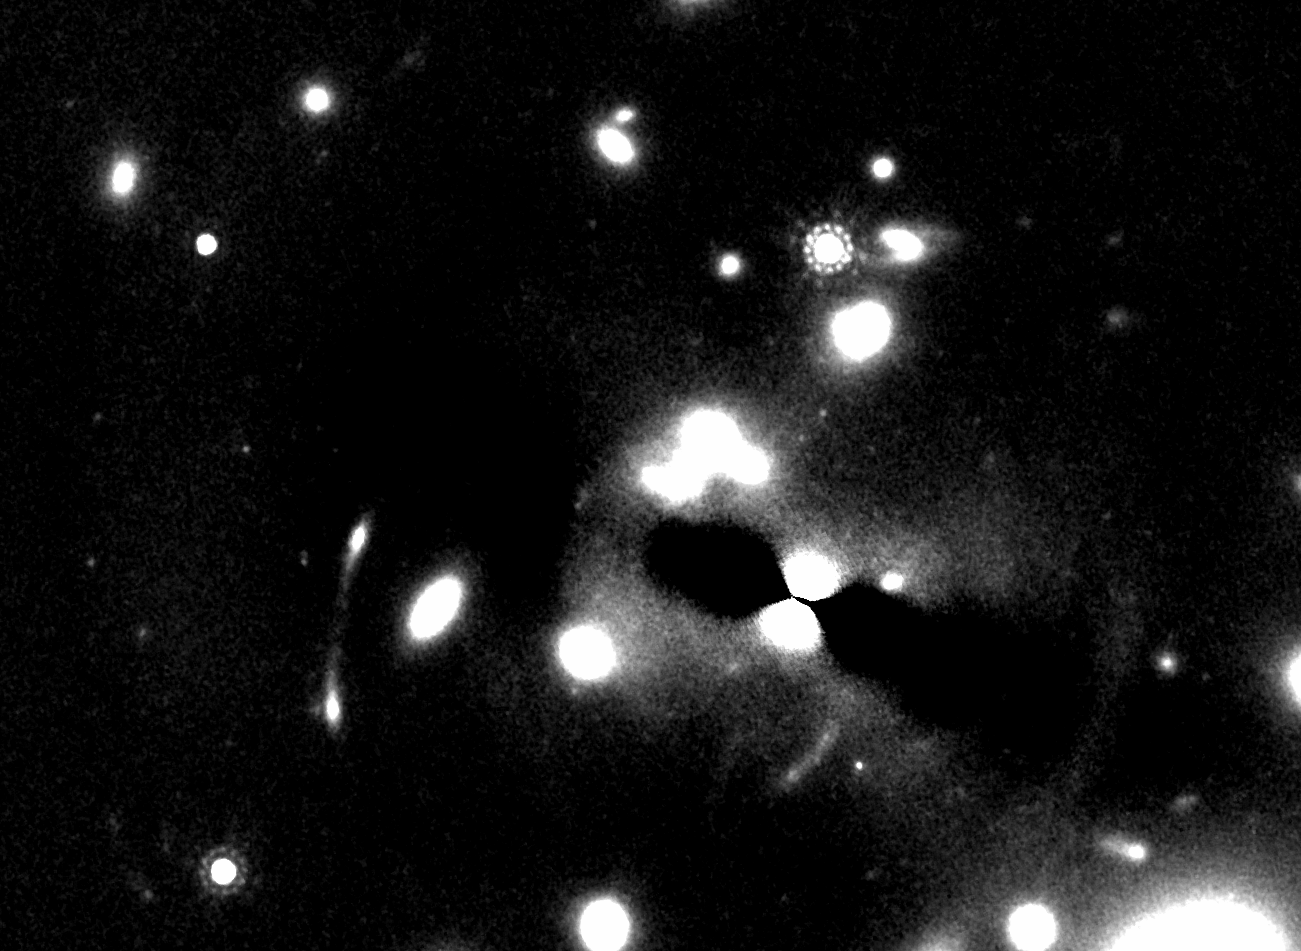
\includegraphics[trim={300 0 0 200}, clip, width=0.5\textwidth]{hst160_sinbcg.png}
\caption{Fila superior, izquierda: imagen de la BCG de \clust{} en el filtro F160W de HST con una escala de 0-0,15 e\(^{-}\)/s. Fila superior, derecha: modelo de GALFIT de la BCG de \clust{}, con la misma escala. En este caso, el modelo es más alargado que la BCG de la imagen original. Inferior: imagen residual resultante de restar la segunda imagen a la primera, con una escala de 0-0,03 e\(^{-}\)/s. El modelo la BCG es claramente inadecuado y no permite distinguir con claridad las estructuras. \label{hst160}}
\end{figure}
\noindent

Esta dificultad obliga a cambiar de estrategia. En lugar de aislar las shells en cada filtro y medir las características de la imagen residual, utilizaremos la imagen del filtro más claro (por lo que ya vimos, F277W de JWST) para identificar las regiones que se corresponden con shells, y haremos todas las mediciones sobre las imágenes originales. La ventaja de este procedimiento, además de la facilidad para extenderlo a todas las imágenes de HST/ACS y MUSE, es la consistencia que otorga el no depender de las variaciones del modelo de la BCG calculado por GALFIT para cada filtro. El principal inconveniente es que las peculiaridades del flujo procedente de las shells pueden ser demasiado sutiles en comparación con el flujo total de la BCG, y por lo tanto podemos estar ocultando características fundamentales. \par

Siguiendo lo expuesto en el párrafo anterior, partimos de la imagen residual de F277W para modelar las formas de los contornos de las shells utilizando la función \textit{measure.find\_contours} de la librería \textit{scikit-image} de Python. En la figura \ref{contours} vemos, marcados en rojo, todos los contornos identificados por el código. De estos, hemos destacado en verde los que verdaderamente se corresponden con shells identificables.\par 

La shell oriental está situada a una distancia galactocéntrica mediana \nota{mejor la media?} de 6,6 arcsec (24,6 kpc) y tiene un área de 34,7 arcsec\(^{2}\) (480,7 kpc\(^{2}\)). Vemos que la parte exterior del contorno está bien definida y se ajusta a lo que esperamos de una shell, con una curvatura amplia pero constante. La única excepción se da en la zona más al sur, en la que una de las galaxias forma un \enquote{bulbo} que extiende la frontera del contorno. En la zona interior, sin embargo, la forma es más compleja. Al norte, las galaxias provocan el mismo fenómeno que acabamos de describir para la frontera exterior, pero de manera aún más acusada. En el centro, el modelo de la galaxia invade parte de la shell y genera una forma de asa, y al sur probablemente no elimina suficientemente la luz de la BCG e identifica como parte de la shell zonas más interiores. Este es esencialmente el mismo problema que teníamos al aplicar el modelo del GALFIT a las imágenes de HST, pero con consecuencias menos graves. Ya que no nos es posible determinar qué partes de la shell son \enquote{verdaderas} y cuáles son un artefacto del modelo, tomaremos este último como referencia y únicamente nos preocuparemos de eliminar la contribución de las galaxias. \par

La shell occidental, por su parte, está más alejada del centro, a una distancia de 9,6 arcsec (35,7 kpc). Como ya esperábamos, es mucho más pequeña, al tener un área de apenas 5,6 arcsec\(^{2}\) (77,6 kpc\(^{2}\)). Su forma es mucho más simple, al no tener ninguna galaxia en su interior ni estar tan cerca del centro galáctico. \par



\begin{figure}[h]
\centering
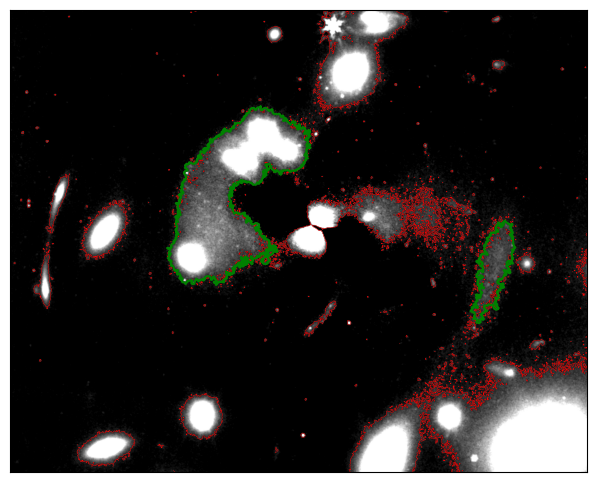
\includegraphics[trim={5 5 5 5}, clip, width=0.6\textwidth]{jwst277_contours.png}
\caption{Definición de los contornos obtenidos por \textit{scikit-image} sobre la tercera imagen de la figura \ref{jwst277}. Destacamos en verde los que se corresponden con shells identificables. Los contornos rojos rodean fundamentalmente otras galaxias. De estas, ayudan especialmente a ver con mayor claridad el \textit{lensing} de la galaxia que se encuentra al sur de la BCG. También se destacan las posibles shells no completas del oeste de la BCG. \label{contours}}
\end{figure}
\noindent

\subsection{Color de las shells} \nota{mover a resultados?} \nota{explicar la conversión a \(m_{AB}\)?}
Una vez caracterizado el contorno de la shell, queremos medir sus propiedades físicas y compararlas con las de otras regiones a la misma distancia galactocéntrica. La primera aproximación que haremos será muy visual. Sabemos que existe una correlación significativa entre el índice de color de una población estelar y su composición química: cuanto mayor es su metalicidad, más roja es una galaxia \citep{bruzualStellarPopulationSynthesis2003,mihosStelLARPOPULATIONSOUTER2013,montesINTRACLUSTERLIGHTFRONTIER2014}. Por ello nos interesa elaborar un mapa de color de la BCG similar al de \citet[fig. 1]{mihosStelLARPOPULATIONSOUTER2013}, comparando el flujo medido por dos de los filtros que tenemos disponibles. No obstante, esta correlación está fuertemente degenerada con la edad de la población estudiada, de modo que una galaxia más antigua también es más roja. En este apartado, por lo tanto, no podemos separar ambos efectos, pero sí es de interés observar, en cualquier caso, si la shell tiene características particulares. \par

Escogemos filtros de HST/ACS para asegurarnos de que no introducimos distorsiones al comparar imágenes de cámaras distintas. De ellos, nos decantamos por F435W y F625W, por generar un contraste suficiente entre sus imágenes y tener anchos de banda similares. En la figura \ref{popmetal}, \citeauthor{popGalaxiesShellsIllustris2017} comparaba la metalicidad mediana de varios puntos situados sobre shells y de otros ajenos a ellas pero situados a las mismas distancias galactocéntricas. En nuestro caso trabajamos con medidas reales en las que, tras la sustracción del fondo, muchos píxeles tienen flujos negativos, por lo que no es posible obtener un valor físicamente válido para el índice de color mediano de un área. Por este motivo reservaremos las medidas numéricas para el apartado siguiente. No obstante, a modo ilustrativo, representamos en el mapa los contornos de las shells, así como varias regiones de referencia con formas idénticas y situadas a las mismas distancias galactocéntricas, rotadas un cierto ángulo con respecto al centro de la BCG calculado por GALFIT. El ángulo es de \(\frac{3\pi}{5}\) en el caso de la shell oriental y de \(\frac{\pi}{3}\) en el caso de la occidental. También incluimos, siguiendo el mismo planteamiento, regiones \enquote{espejo} situadas en el extremo opuesto de la BCG para cada shell. En la figura \ref{color} vemos el mapa de color con los contornos de las shells representados en blanco, las regiones de referencia en naranja, y las regiones espejo en verde. Sobre ella se ha aplicado, con el objetivo de reducir el ruido visual de la imagen, un filtro gaussiano con la función \textit{ndimage.gaussian\_filter} de la librería de Python \textit{scipy} con \(\textit{sigma} = 0,6\). \nota{puede que no ayude} \par % ya que hacemos un ejercicio similar, pero, dado que estamos trabajando con una imagen real y necesitamos áreas mayores, utilizamos toda la superficie de las shells (con las galaxias enmascaradas) calculada en los apartados anteriores y medimos el índice de color F435W - F625W sobre ellas. las áreas sin shells utilizamos contornos de idéntica forma y situados a la misma distancia al centro galáctico, con una rotación con respecto a este de \(\frac{3\pi}{5}\) en el caso de la shell oriental y \(\frac{\pi}{3}\) en el de la occidental.


\begin{figure}[h]
\centering
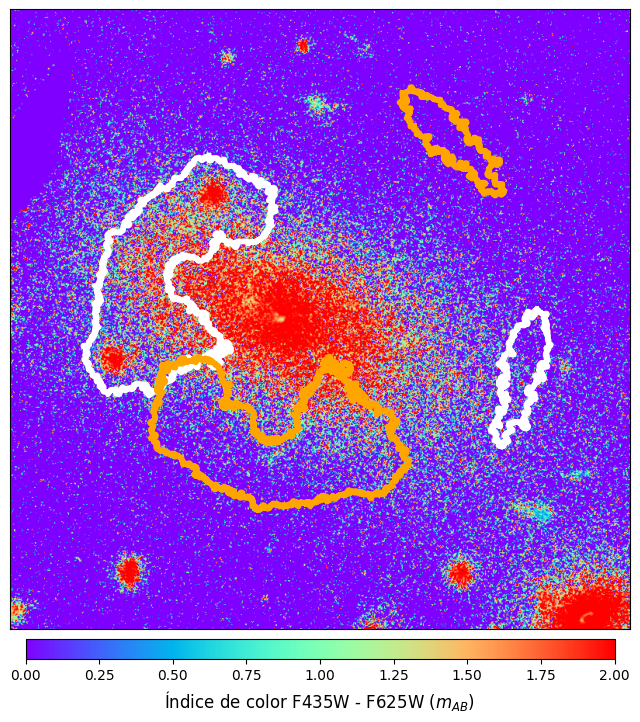
\includegraphics[trim={5 0 5 5}, clip, width=0.7\textwidth]{color.png}
\caption{\nota{escribir pie de figura} \nota{meter contornos espejo}\label{color}}
\end{figure}
\noindent

Es evidente que las regiones más rojas son las cercanas a los centros galácticos, lo que ya era esperable y se apreciaba de forma nítida en \citet[fig. 1]{mihosStelLARPOPULATIONSOUTER2013}. En cuanto a las shells, observamos un claro exceso de luminosidad del filtro rojo en la zona perteneciente a la shell oriental, especialmente en comparación con su región de referencia. Su región espejo también es visiblemente más azul, por lo que, si existen shells en esta zona que no pudimos detectar, estas no exhiben las mismas propiedades. Más al oeste, en la shell pequeña, el índice de color no es especialmente alto, pero sí destaca frente a su región de referencia al norte. \nota{incluir región espejo pequeña} Todo esto parece indicar que, como indicaban las predicciones teóricas, las shells presentan un exceso de luminosidad en los filtros más rojos. \par

%Las medidas confirman estas apreciaciones. El índice de color mediano en el contorno de la shell, con las galaxias enmascaradas como se indica en el apartado \ref{sec:mascara}, es de 1,65, mientras que en la región de referencia (también enmascarada en lugares equivalentes) es de 1,32. 

\subsection{Análisis espectroscópico y fotométrico de la shell oriental}
\nota{descripción de los objetivos}
\subsubsection{Selección de la región de estudio} \label{sec:mascara}
En el apartado \ref{sec:contorno} describimos la morfología de las dos shells que pudimos identificar en la imagen tomada con el filtro F277W de JWST. El siguiente paso consiste en seleccionar la región sobre la que haremos los análisis fotométrico y espectroscópico. Debido a su pequeño tamaño y baja luminosidad, la shell occidental puede presentar dificultades para su estudio. Por lo tanto, en lo que resta de este trabajo nos centraremos en la shell oriental. \par

No obstante, como señalamos en el apartado \ref{sec:galaxias} y la figura \ref{fig:galaxias}, en la shell oriental están presentes varias galaxias que no podemos incluir en el análisis. El procedimiento más sencillo para eliminar su influencia en las propiedades de la shell es aplicar una máscara sobre la región en la que se encuentran. El inconveniente de este enfoque es que corremos el riesgo de reducir en exceso el área de estudio y, como consecuencia de ello, trabajar con un flujo excesivamente bajo y dificultar la obtención de resultados concluyentes. Por ello la máscara debe ser mínima. \par

\nota{puedo incluir los intentos de eliminar las galaxias de la shell con GALFIT y CHEFs o no. es cierto que no lleva a nada}

\begin{comment}
\begin{figure}[h]
\centering
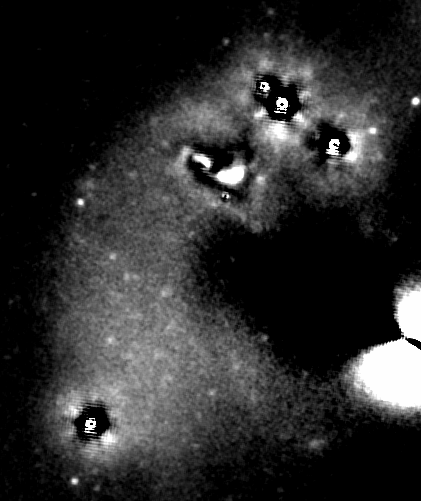
\includegraphics[trim={0 0 0 0}, clip, width=0.4\textwidth]{galaxiasgalfit.png}
\caption{\nota{escribir pie de figura. PSF?} 0-0,2 MJy/sr \label{fig:galgalfit}}
\end{figure}
\noindent
\end{comment}

Para evaluar si una máscara es adecuada, tomamos como referencia una región en el centro de la shell situada entre \(+00^{\circ} 05^{\prime}22^{\prime\prime}.12\) y \(+00^{\circ} 05^{\prime}23^{\prime\prime}.32\) de declinación y con un área de 3,2 arcsec\(^{2}\) (44,3 kpc\(^{2}\)). Esta región no se ve afectada por la influencia de las galaxias. Posteriormente se compara el flujo de la shell enmascarada en cada filtro \nota{qué filtros?} con el de la región de referencia. Si \nota{procedimiento para averiguar similitud}, la máscara se considera apta para medir las propiedades de la shell. \par

\nota{descripción más en detalle de la medición del flujo} \nota{paso de las máscaras a otros telescopios}
La medición del flujo en la shell se hará en maggies, donde el flujo en maggies \(\Phi_{mag} = 10^{-0,4 m_{AB}}\), siendo \(m_{AB}\) la magnitud AB del objeto\footnote{\url{https://prospect.readthedocs.io/en/latest/dataformat.html}}. También es necesario considerar las fuentes de error de la imagen. Existen dos principales: la incertidumbre de Poisson asociada al número de cuentas medido por el detector y el ruido de fondo de la imagen. A su vez, el ruido de fondo está compuesto por la incertidumbre en \nota{sky noise in the aperture?}, y por \nota{aperture sum?}. \par

La máscara calculada


\subsubsection{Obtención de propiedades físicas y químicas}
\nota{descripción de CIGALE}

